\section{Nondeterministic automata}

A right-linear grammar may include two alternative rules starting with the same character. 
This implies that in state $A$, upon reading the character, the machine can decide which of the subsequent states to enter, introducing non-determinism in its behavior.
A machine move that does not read an input character is referred to as a spontaneous or epsilon move. 
These spontaneous moves also contribute to the nondeterministic nature of the machine.
The primary advantages of nondeterminism are:
\begin{itemize}
    \item The correspondence between grammars and automata suggests the inclusion of:
        \begin{itemize}
            \item Moves with two or more destination states.
            \item Spontaneous moves (or $\varepsilon$-moves).
            \item Two or more initial states.
        \end{itemize}
    \item Conciseness: defining a language using a nondeterministic automaton can often be more readable and compact compared to using a deterministic one.
\end{itemize}

\paragraph*{Nondeterministic finite state automaton}
A nondeterministic finite automaton $N$, excluding spontaneous moves, is characterized by the following components:
\begin{itemize}
    \item The state set $Q$. 
    \item The terminal alphabet $\Sigma$. 
    \item Two subsets of $Q$: the set $I$ of the initial states and the set $F$ of final states.
    \item The transition relation $\delta$, a subset of the Cartesian product $Q\times\Sigma\times Q$.     
\end{itemize}
A computation of length $n$ initiates at state $q_0$ and concludes at state $q_n$, with the labeling $a_1a_2\dots a_n$. 
\begin{definition}[\textit{Acceptance condition}]
    An input string $x$ is accepted by the automaton if it represents the labeling of a path that begins at an initial state and concludes at a final state:
    \[L(N)=\{x \in \Sigma^{*}|q \overset{x}{\rightarrow} \textnormal{ with } q \in I \textnormal{ and } r \in F\}\]
\end{definition}
The moves of the nondeterministic automaton can be defined through a many-valued transition function.  
For a machine $N=(Q,\Sigma,\delta,I,F)$, without spontaneous moves, the transition function $\delta$ is defined to have the domain and image:
\[\delta:Q\times\left(\Sigma\cup\{\varepsilon\}\right)\rightarrow \wp(Q)\]
where the symbol $\wp(Q)$ denotes the power set of the set $Q$.
A nondeterministic automaton may possess two or more initial states.
However, constructing an equivalent nondeterministic automaton with only one initial state is straightforward.
Introduce a new initial state $q_0$, connect it to the existing initial states through $\varepsilon$-arcs, designate these states as non-initial, and retain only $q_0$ as the initial state.

\subsection{Correspondence between automata and grammars}
Consider a strictly right-linear grammar $G=(V,\Sigma,P,S)$ and a nondeterministic automaton $N=(Q,\Sigma,\delta,q_0,F)$ with a unique initial state.
The following equivalences hold:
\begin{table}[H]
    \centering
    \begin{tabular}{cc}
    \hline
    \textbf{Right-linear grammar}                            & \textbf{Finite state automaton} \\ \hline
    Nonterminal set $V$                                      & Set of states $Q=V$             \\
    Axiom $S=q_0$                                            & Initial state $q_0=S$           \\
    $p \rightarrow aq$, where $a \in \Sigma$ and $p,q \in V$ & \begin{minipage}{.2\textwidth}\centering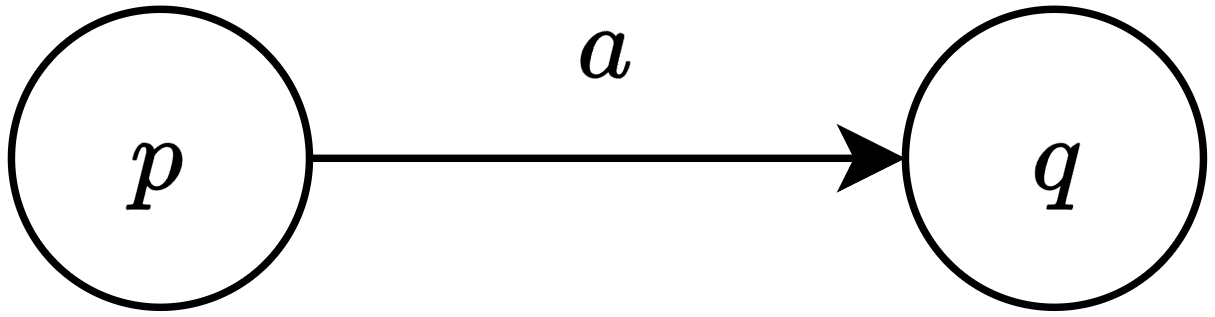
\includegraphics[width=\linewidth, height=9mm]{images/a.png}\end{minipage}                                \\
    $p \rightarrow q$, where $p,q \in V$                     & \begin{minipage}{.2\textwidth}\centering
\includegraphics[width=\linewidth, height=9mm]{images/b.png}\end{minipage}                                 \\
    $p \rightarrow a$, where $p,a \in V$ (terminal rule)     & \begin{minipage}{.2\textwidth}\centering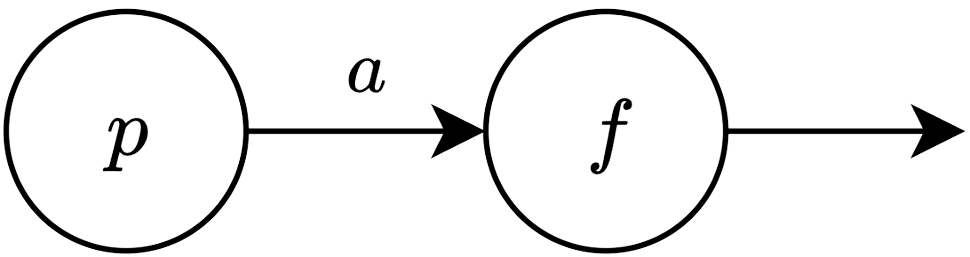
\includegraphics[width=\linewidth, height=9mm]{images/c.png}\end{minipage}                                 \\
    $p \rightarrow \varepsilon$                              & Final state $p$                 \\ \hline
    \end{tabular}
\end{table}
\begin{example}
    Consider the following nondeterministic automaton:
    \begin{figure}[H]
        \centering
        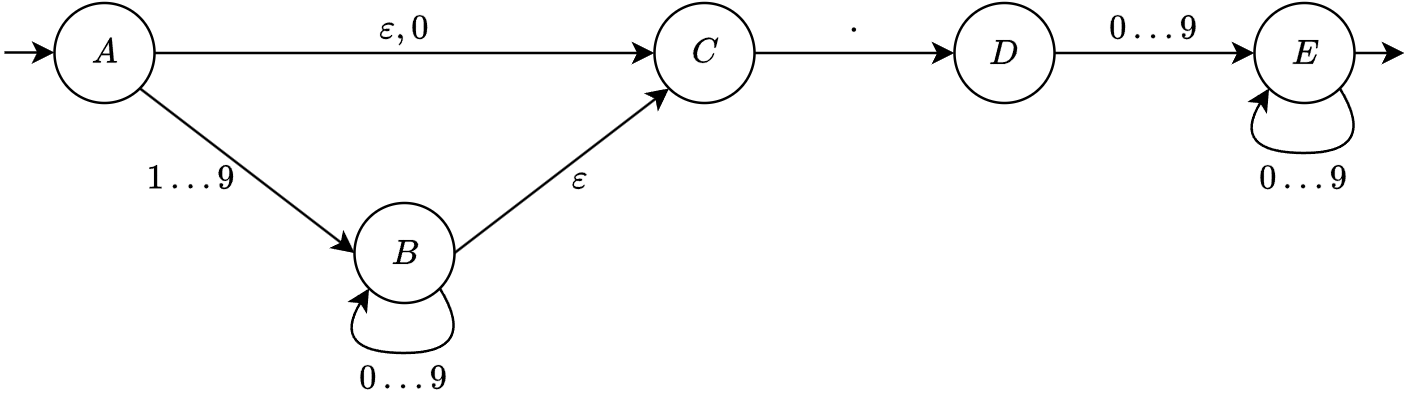
\includegraphics[width=0.75\linewidth]{images/nfsa.png}
    \end{figure}
    It can be easily translated into a grammar following the rules in the table above:
    \[\begin{cases}
        A \rightarrow 0C|C|1B|\dots|9B \\
        B \rightarrow 0B|\dots|9B|C \\
        C \rightarrow \cdot D \\
        D \rightarrow 0E|\dots|9E \\
        E \rightarrow 0E|\dots|9E|\varepsilon
    \end{cases}\]
\end{example}
As a result, a grammar derivation corresponds to an automaton computation, and vice versa.
\begin{proposition}
    A language is generated by a right-linear grammar if and only if it is recognized by a finite automaton.
\end{proposition}

\subsection{Ambiguity}
Grammar derivations have a one-to-one correspondence with automaton computations, extending ambiguity from grammars to automata.
\begin{definition}[\textit{Ambiguous automaton}]
    An automaton is considered ambiguous if, and only if, the corresponding grammar exhibits ambiguity. 
\end{definition}
In other words, if a string $x$ labels two or more accepting paths in the automaton.
It is evident from the definition that a deterministic automaton is never ambiguous. 
Regular language families can also be defined using left-linear grammars. 
By substituting left for right, the mapping between such grammars and automata can be easily established.